\hypertarget{hypertext-transfer-protocol}{%
\section{HyperText Transfer
Protocol}\label{hypertext-transfer-protocol}}

\begin{itemize}
\tightlist
\item
  Protocole application : invention www en 1990 (v0.9)

  \begin{itemize}
  \tightlist
  \item
    Connexion, GET, réponse, fermeture
  \end{itemize}
\item
  HTTP 1.0 (1996)

  \begin{itemize}
  \tightlist
  \item
    Entêtes de requête (Host, Referer, User-Agent, \ldots{})
  \item
    Entêtes de réponse (Content-Type, Set-Cookie, Location, \ldots{})
  \end{itemize}
\item
  HTTP 1.1 (1997)

  \begin{itemize}
  \tightlist
  \item
    Keep-alive, pipelining, cache, \ldots{}
  \item
    Plus d'entêtes, Host obligatoire
  \end{itemize}
\item
  \href{https://docs.google.com/presentation/d/1eqae3OBCxwWswOsaWMAWRpqnmrVVrAfPQclfSqPkXrA/present\#slide=id.p19}{HTTP
  2.0} (2015)

  \begin{itemize}
  \tightlist
  \item
    Binaire, multiplexage connexions, compresions entêtes, push,
    \ldots{}
  \item
    Supporté par \href{http://caniuse.com/\#feat=http2}{presque tous}
    les navigateurs, une majorité de serveurs
  \end{itemize}
\end{itemize}

\hypertarget{codes-de-ruxe9ponse}{%
\section{Codes de réponse}\label{codes-de-ruxe9ponse}}

\begin{itemize}
\tightlist
\item
  1xx : Information
\item
  2xx : Succès
\item
  3xx : Redirection
\item
  4xx : Erreur Client
\item
  5xx : Erreur Serveur
\end{itemize}

\hypertarget{muxe9thodes-http-verbes}{%
\section{Méthodes HTTP (verbes)}\label{muxe9thodes-http-verbes}}

\begin{itemize}
\tightlist
\item
  {GET} : Demander une ressource
\item
  POST : Création d'une ressource
\item
  {PUT} : Remplacement total d'une ressource
\item
  PATCH : Remplacement partiel d'une ressource
\item
  {DELETE} : Suppression d'une ressource
\item
  {HEAD} : Demande l'entête de la réponse, sans la ressource
\item
  {TRACE, OPTIONS}, CONNECT
\end{itemize}

{idempotentes} {sûres}

\hypertarget{echanges-http}{%
\section{Echanges HTTP}\label{echanges-http}}

\begin{itemize}
\tightlist
\item
  Requête
\end{itemize}

\begin{otherlanguage}{english}

\begin{Shaded}
\begin{Highlighting}[]
\NormalTok{GET / HTTP/1.1[CRLF]}
\NormalTok{Host: www.cff.ch[CRLF]}
\NormalTok{Connection: close[CRLF]}
\NormalTok{User-Agent: Opera/9.20 (Windows NT 6.0; U; en)[CRLF]}
\NormalTok{Accept-Encoding: gzip[CRLF]}
\NormalTok{Accept-Charset: ISO-8859-1,UTF-8;q=0.7,*;q=0.7[CRLF]}
\NormalTok{Cache-Control: no[CRLF]}
\NormalTok{Accept-Language: de,en;q=0.7,en-us;q=0.3[CRLF]}
\NormalTok{Referer: http://web-sniffer.net/[CRLF]}
\NormalTok{[CRLF]}
\end{Highlighting}
\end{Shaded}

\end{otherlanguage}

\begin{itemize}
\tightlist
\item
  Réponse
\end{itemize}

\begin{otherlanguage}{english}

\begin{Shaded}
\begin{Highlighting}[]
\NormalTok{HTTP Status Code:   HTTP/1.1 302 Found}
\NormalTok{Date:           Mon, 16 Nov 2009 08:01:35 GMT   }
\NormalTok{Server:         Apache  }
\NormalTok{Location:       http://www.sbb.ch/fr/   }
\NormalTok{Content-Length:     205 }
\NormalTok{Connection:     close   }
\NormalTok{Content-Type:       text/html; charset=iso-8859-1}

\DataTypeTok{<!DOCTYPE }\NormalTok{HTML PUBLIC "-//IETF//DTD HTML 2.0//EN"}\DataTypeTok{>}
\KeywordTok{<html><head><title>}\NormalTok{302 Found}\KeywordTok{</title>}
\KeywordTok{</head><body>}
\KeywordTok{<h1>}\NormalTok{Found}\KeywordTok{</h1>}
\KeywordTok{<p>}\NormalTok{The document has moved }\KeywordTok{<a}\OtherTok{ href=}\StringTok{"http://www.sbb.ch/fr/"}\KeywordTok{>}\NormalTok{here}\KeywordTok{</a>}\NormalTok{.}\KeywordTok{</p>}
\KeywordTok{</body></html>}
\end{Highlighting}
\end{Shaded}

\end{otherlanguage}

\hypertarget{http}{%
\section{HTTP}\label{http}}

\begin{itemize}
\tightlist
\item
  Requête POST : paramètres dans le corps
\end{itemize}

\begin{otherlanguage}{english}

\begin{Shaded}
\begin{Highlighting}[]
\NormalTok{POST /login.jsp HTTP/1.1}
\NormalTok{Host: www.mysite.com}
\NormalTok{User-Agent: Mozilla/4.0}
\NormalTok{Content-Length: 27}
\NormalTok{Content-Type: application/x-www-form-urlencoded}

\NormalTok{userid=joe}\ErrorTok{&}\NormalTok{password=guessme}
\end{Highlighting}
\end{Shaded}

\end{otherlanguage}

\begin{itemize}
\tightlist
\item
  Outils HTTP

  \begin{itemize}
  \tightlist
  \item
    CLI : curl
  \item
    Browser dev tools
  \item
    WebApp : \href{http://hurl.it/}{HURL}
  \end{itemize}
\item
  Exemples PATCH :
  \href{http://www.mnot.net/blog/2012/09/05/patch}{mnot} ,
  \href{http://soabits.blogspot.ch/2013/01/http-put-patch-or-post-partial-updates.html}{SOA
  bits}
\end{itemize}

\hypertarget{ajax-historique}{%
\section{AJAX : Historique}\label{ajax-historique}}

\begin{itemize}
\tightlist
\item
  Asynchronous Javascript And Xml
\item
  Buzzword,
  \href{http://web.archive.org/web/20110102130434/http://www.adaptivepath.com/ideas/essays/archives/000385.php}{Jesse
  James Garret}, 2005
\item
  Mise à jour sans rechargement intégral
\item
  Utilisation de
  \href{https://en.wikipedia.org/wiki/Remote_scripting}{Remote
  Scripting} et de DOM
\item
  Historique de techniques de remote scripting

  \begin{itemize}
  \tightlist
  \item
    \href{http://archive.oreilly.com/pub/a/javascript/2002/02/08/iframe.html}{(i)frames}
  \item
    Bibliothèques JS (ex:
    \href{http://www.ashleyit.com/rs/jsrs/test.htm}{JSRS})
  \item
    Utilisation des images/cookies (ex:
    \href{http://web.archive.org/web/20100916110710/http://depressedpress.com/Content/Development/JavaScript/Articles/GIFAsPipe/Index.cfm}{GIF})
  \item
    Applets, Flash, ActiveX, \ldots{}
  \item
    {XHR : XML HTTP Request} (IE5, 1999 pour OWA)
  \item
    Fetch API
  \end{itemize}
\item
  Pas obligatoire d'avoir du JS, XML ni d'être asynchrone !
\end{itemize}

\hypertarget{ajax}{%
\section{AJAX}\label{ajax}}

\begin{itemize}
\tightlist
\item
  XHR est devenue la méthode standard

  \begin{itemize}
  \tightlist
  \item
    Popularisée par Google (GMaps, GMail, \ldots{})
  \item
    Le w3c fait évoluer un
    \href{https://www.w3.org/TR/XMLHttpRequest/}{draft} depuis 2006
  \end{itemize}
\item
  Principe

  \begin{enumerate}
  \def\labelenumi{\arabic{enumi}.}
  \tightlist
  \item
    Envoi de requête HTTP
  \item
    La réponse provoque l'éxecution de la fonction de rappel
  \item
    Le DOM de la page est mis à jour
  \end{enumerate}
\item
  Applications

  \begin{itemize}
  \tightlist
  \item
    GUI ressemblant à des app natives
  \item
    MAJ dynamiques de formulaires, autocompletion
  \item
    Validation avec interrogation du serveur
  \item
    \ldots{}
  \end{itemize}
\end{itemize}

\hypertarget{lobjet-xmlhttprequest}{%
\section{\texorpdfstring{L'objet
\emph{XMLHttpRequest}}{L'objet XMLHttpRequest}}\label{lobjet-xmlhttprequest}}

\begin{itemize}
\tightlist
\item
  Initiative de Microsoft

  \begin{itemize}
  \tightlist
  \item
    Composant ActiveX de IE5
  \item
    Adopté par Mozilla 1.0 et Safari 1.2
  \item
    Standardisation W3C en cours
  \end{itemize}
\item
  Requête HTTP en JS
\item
  Fonction de rappel (callback)
\item
  Asynchrone : Non bloquant
\item
  Non standard =\textgreater{} différentes implémentations
\item
  Supporté par Chrome, FF, Safari, IE, Konqueror, \ldots{}
\item
  Alternative souhaitable si JS désactivé
\end{itemize}

\hypertarget{xhr-en-js}{%
\section{XHR en JS}\label{xhr-en-js}}

\begin{otherlanguage}{english}

\begin{Shaded}
\begin{Highlighting}[]
\KeywordTok{var}\NormalTok{ xhr}\OperatorTok{;}
\KeywordTok{function} \AttributeTok{createXMLHttpRequest}\NormalTok{() }
\OperatorTok{\{}
    \ControlFlowTok{if}\NormalTok{ (}\VariableTok{window}\NormalTok{.}\AttributeTok{ActiveXObject}\NormalTok{) }
    \OperatorTok{\{}
\NormalTok{        xhr }\OperatorTok{=} \KeywordTok{new} \AttributeTok{ActiveXObject}\NormalTok{(}\StringTok{"Microsoft.XMLHTTP"}\NormalTok{)}\OperatorTok{;}
    \OperatorTok{\}}
    \ControlFlowTok{else} \ControlFlowTok{if}\NormalTok{ (}\VariableTok{window}\NormalTok{.}\AttributeTok{XMLHttpRequest}\NormalTok{) }
    \OperatorTok{\{}
\NormalTok{        xhr }\OperatorTok{=} \KeywordTok{new} \AttributeTok{XMLHttpRequest}\NormalTok{()}\OperatorTok{;}
    \OperatorTok{\}}
\OperatorTok{\}}
\end{Highlighting}
\end{Shaded}

\end{otherlanguage}

\begin{itemize}
\tightlist
\item
  Dans son
  \href{http://www.xul.fr/xml-ajax.html\#ajax-exemple}{contexte}
\end{itemize}

\hypertarget{xhr-en-jquery-avec-load}{%
\section{\texorpdfstring{XHR en jQuery avec
\emph{load()}}{XHR en jQuery avec load()}}\label{xhr-en-jquery-avec-load}}

\begin{otherlanguage}{english}

\begin{Shaded}
\begin{Highlighting}[]
\DataTypeTok{<!DOCTYPE }\NormalTok{html}\DataTypeTok{>}
\KeywordTok{<html>}
\KeywordTok{<head>}
\KeywordTok{<script}\OtherTok{ src=}\StringTok{"jquery.js"}\KeywordTok{></script>}
\KeywordTok{<script>}
\AttributeTok{$}\NormalTok{(document).}\AttributeTok{ready}\NormalTok{(}\KeywordTok{function}\NormalTok{()}\OperatorTok{\{}
  \AttributeTok{$}\NormalTok{(}\StringTok{"button"}\NormalTok{).}\AttributeTok{click}\NormalTok{(}\KeywordTok{function}\NormalTok{()}\OperatorTok{\{}
    \AttributeTok{$}\NormalTok{(}\StringTok{"#div1"}\NormalTok{).}\AttributeTok{load}\NormalTok{(}\StringTok{"demo_test.txt"}\NormalTok{)}\OperatorTok{;}
  \OperatorTok{\}}\NormalTok{)}\OperatorTok{;}
\OperatorTok{\}}\NormalTok{)}\OperatorTok{;}
\KeywordTok{</script>}
\KeywordTok{</head>}

\KeywordTok{<body>}
  \KeywordTok{<div}\OtherTok{ id=}\StringTok{"div1"}\KeywordTok{><h2>}\NormalTok{Let jQuery AJAX Change This Text}\KeywordTok{</h2></div>}
  \KeywordTok{<button>}\NormalTok{Get External Content}\KeywordTok{</button>}
\KeywordTok{</body>}
\KeywordTok{</html>}
\end{Highlighting}
\end{Shaded}

\end{otherlanguage}

\begin{itemize}
\tightlist
\item
  \href{http://www.w3schools.com/jquery/tryit.asp?filename=tryjquery_ajax_load}{Tester}
\item
  D'\href{https://code.tutsplus.com/tutorials/jquery-succinctly-jquery-and-ajax--net-33856}{autres}
  façons de faire
\end{itemize}

\hypertarget{xhr-propriuxe9tuxe9s-et-muxe9thodes}{%
\section{XHR : propriétés et
méthodes}\label{xhr-propriuxe9tuxe9s-et-muxe9thodes}}

\begin{itemize}
\tightlist
\item
  \begin{otherlanguage}{english}\texttt{readyState,\ status,\ onreadystatechange}\end{otherlanguage}
\item
  \begin{otherlanguage}{english}\texttt{responseText,\ responseXML}\end{otherlanguage}
\item
  \begin{otherlanguage}{english}\texttt{open\ (Verbe,\ URI,\ async)\ :}\end{otherlanguage}

  \begin{itemize}
  \tightlist
  \item
    \begin{otherlanguage}{english}\texttt{Verbe}\end{otherlanguage} HTTP
    : ``GET'', ``POST'' ou ``PUT''
  \item
    \begin{otherlanguage}{english}\texttt{URI}\end{otherlanguage} :
    destinataire de la requête
  \item
    \begin{otherlanguage}{english}\texttt{async}\end{otherlanguage}
    (bool) :
    \begin{otherlanguage}{english}\texttt{true}\end{otherlanguage} =
    asynchrone,
    \begin{otherlanguage}{english}\texttt{false}\end{otherlanguage} =
    bloquant
  \end{itemize}
\item
  \begin{otherlanguage}{english}\texttt{send\ (null\ \textbar{}\ string)}\end{otherlanguage}
  : peut être bloquante
\item
  \begin{otherlanguage}{english}\texttt{setRequestHeader(header,\ value)}\end{otherlanguage}
\item
  \begin{otherlanguage}{english}\texttt{getResponseHeader(string)}\end{otherlanguage}
\item
  \begin{otherlanguage}{english}\texttt{abort()}\end{otherlanguage}
\end{itemize}

\hypertarget{envoi-de-donnuxe9es}{%
\section{Envoi de données}\label{envoi-de-donnuxe9es}}

\begin{itemize}
\tightlist
\item
  GET

  \begin{itemize}
  \tightlist
  \item
    {Obtenir des données}
  \item
    Longueur URL limitée par le navigateur (2'048 pour IE)
  \item
    Utilise le cache (navigateur, proxy)
  \item
    manipulables par l'utilisateur (bookmarks, partage, \ldots{})
  \end{itemize}
\item
  POST

  \begin{itemize}
  \tightlist
  \item
    {Faire quelque chose}
  \item
    Données sensibles
  \item
    Longueur limitée par le serveur (assez large)
  \item
    Utilisation de la méthode send() de XHR
  \item
    Requête Ajax en 2 temps (entête, puis données)
  \end{itemize}
\item
  Cache

  \begin{itemize}
  \tightlist
  \item
    Client : Construire des
    \href{http://stackoverflow.com/questions/367786/prevent-browser-caching-of-jquery-ajax-call-result}{URL
    uniques}
  \item
    Serveur : Envoi
    d'\href{https://developers.google.com/web/fundamentals/performance/optimizing-content-efficiency/http-caching}{entêtes}
    interdisant le cache
  \end{itemize}
\end{itemize}

\begin{otherlanguage}{english}

\begin{Shaded}
\begin{Highlighting}[]
\VariableTok{MyXhr}\NormalTok{.}\AttributeTok{open}\NormalTok{(}\StringTok{"GET"}\OperatorTok{,} \StringTok{"fichier.xml"}\OperatorTok{,} \KeywordTok{true}\NormalTok{)}\OperatorTok{;}
\VariableTok{MyXhr}\NormalTok{.}\AttributeTok{setRequestHeader}\NormalTok{(}\StringTok{"Cache-Control"}\OperatorTok{,} \StringTok{"no-store, no-cache, must-revalidate, }
\NormalTok{            post}\OperatorTok{-}\NormalTok{check}\OperatorTok{=}\DecValTok{0}\OperatorTok{,}\NormalTok{ pre}\OperatorTok{-}\NormalTok{check}\OperatorTok{=}\DecValTok{0}\StringTok{");}
\VariableTok{MyXhr}\NormalTok{.}\AttributeTok{setRequestHeader}\NormalTok{(}\StringTok{"Pragma"}\OperatorTok{,} \StringTok{"no-cache"}\NormalTok{)}\OperatorTok{;}
\VariableTok{MyXhr}\NormalTok{.}\AttributeTok{setRequestHeader}\NormalTok{(}\StringTok{"Expires"}\OperatorTok{,} \StringTok{"Wed, 09 Aug 2000 08:21:57 GMT"}\NormalTok{)}\OperatorTok{;} 
\end{Highlighting}
\end{Shaded}

\end{otherlanguage}

\hypertarget{pruxe9fuxe9rer-get-sauf}{%
\section{Préférer GET, sauf}\label{pruxe9fuxe9rer-get-sauf}}

\begin{figure}
\centering
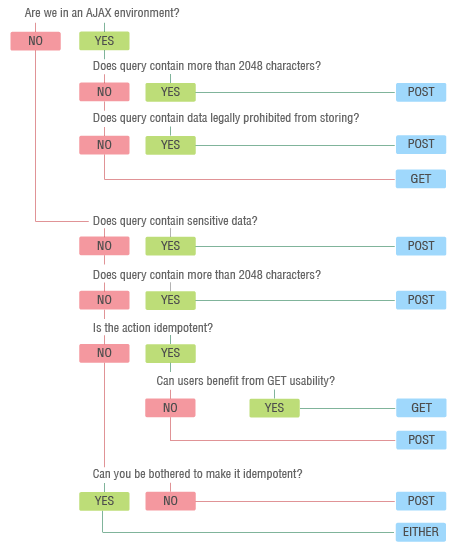
\includegraphics{src/img/GETvsPOST.png}
\caption{``GETorPOST''}
\end{figure}

\href{http://blog.teamtreehouse.com/the-definitive-guide-to-get-vs-post}{Détails}

\hypertarget{ruxe9ponse-en-texte}{%
\section{Réponse en texte}\label{ruxe9ponse-en-texte}}

\begin{itemize}
\tightlist
\item
  Si la requête aboutit :

  \begin{itemize}
  \tightlist
  \item
    \begin{otherlanguage}{english}\texttt{readystate\ ==\ 4}\end{otherlanguage}
  \item
    \begin{otherlanguage}{english}\texttt{status\ ==\ 200}\end{otherlanguage}
  \end{itemize}
\item
  La réponse est dans l'attribut
  \begin{otherlanguage}{english}\texttt{responseText}\end{otherlanguage}
\item
  ou dans
  \begin{otherlanguage}{english}\texttt{responseXML}\end{otherlanguage}

  \begin{itemize}
  \tightlist
  \item
    Utilisation du DOM
    (\begin{otherlanguage}{english}\texttt{getElementsByTagName(),\ ...}\end{otherlanguage})
  \end{itemize}
\end{itemize}

\hypertarget{ruxe9ponse-en-xml}{%
\section{Réponse en XML}\label{ruxe9ponse-en-xml}}

\begin{otherlanguage}{english}

\begin{Shaded}
\begin{Highlighting}[]
\KeywordTok{<?xml}\NormalTok{ version="1.0" }\KeywordTok{?>}
\KeywordTok{<liste>}
     \KeywordTok{<personne>}
         \KeywordTok{<nom>}\NormalTok{Berger}\KeywordTok{</nom>}
         \KeywordTok{<prenom>}\NormalTok{Laurent}\KeywordTok{</prenom>}
     \KeywordTok{</personne>}
     \KeywordTok{<personne>}
         \KeywordTok{<nom>}\NormalTok{Borgo}\KeywordTok{</nom>}
         \KeywordTok{<prenom>}\NormalTok{Sébastien}\KeywordTok{</prenom>}
     \KeywordTok{</personne>}
     \KeywordTok{<personne>}
         \KeywordTok{<nom>}\NormalTok{Bux}\KeywordTok{</nom>}
         \KeywordTok{<prenom>}\NormalTok{Rémy}\KeywordTok{</prenom>}
     \KeywordTok{</personne>}
\KeywordTok{</liste>}
\end{Highlighting}
\end{Shaded}

\end{otherlanguage}

\begin{itemize}
\tightlist
\item
  Dans
  \begin{otherlanguage}{english}\texttt{responseXML}\end{otherlanguage}
\end{itemize}

\hypertarget{ruxe9ponse-en-json19}{%
\section{\texorpdfstring{Réponse en
\href{http://www.json.org/}{JSON}}{Réponse en JSON}}\label{ruxe9ponse-en-json19}}

\begin{itemize}
\tightlist
\item
  \href{http://www.ecma-international.org/publications/files/ECMA-ST/ECMA-404.pdf}{Standard}
  depuis octobre 2013 (\href{http://www.crockford.com/}{Douglas
  Crockford})
\item
  Tableau d'objets js :

  \begin{itemize}
  \tightlist
  \item
    pour chacun, ses attributs sont des paires clé:valeur
  \end{itemize}
\end{itemize}

\begin{otherlanguage}{english}

\begin{Shaded}
\begin{Highlighting}[]
\FunctionTok{\{}\ErrorTok{objet1} \FunctionTok{:} \ErrorTok{nom} \ErrorTok{:} \ErrorTok{'Berger'}\FunctionTok{,} \ErrorTok{prenom}\FunctionTok{:} \ErrorTok{'Laurent'}\FunctionTok{\}}

\OtherTok{[}\ErrorTok{objet1}\OtherTok{,} \ErrorTok{objet2}\OtherTok{,} \ErrorTok{objet3}\OtherTok{]}

\OtherTok{[}
    \FunctionTok{\{}\ErrorTok{nom}\FunctionTok{:}\StringTok{"Berger"}\FunctionTok{,}  \ErrorTok{prenom}\FunctionTok{:}\StringTok{"Laurent"}\FunctionTok{\}}\OtherTok{,}
    \FunctionTok{\{}\ErrorTok{nom}\FunctionTok{:}\StringTok{"Borgo"}\FunctionTok{,}   \ErrorTok{prenom}\FunctionTok{:}\StringTok{"Sébastien"}\FunctionTok{\}}\OtherTok{,}
    \FunctionTok{\{}\ErrorTok{nom}\FunctionTok{:}\StringTok{"Bux"}\FunctionTok{,}     \ErrorTok{prenom}\FunctionTok{:}\StringTok{"Rémy"}\FunctionTok{\}}
\OtherTok{]}
\end{Highlighting}
\end{Shaded}

\end{otherlanguage}

\begin{itemize}
\tightlist
\item
  Utilisation de :
  \begin{otherlanguage}{english}\texttt{\textasciitilde{}\textasciitilde{}var\ users\ =\ eval(\textquotesingle{}(\textquotesingle{}\ +\ myXHR.responseText\ +\ \textquotesingle{})\textquotesingle{});\ \textasciitilde{}\textasciitilde{}}\end{otherlanguage}
  pour créer le tableau d'objets correspondant
\end{itemize}

\hypertarget{eval-is-evil-22}{%
\section{\texorpdfstring{\href{https://javascriptweblog.wordpress.com/2010/04/19/how-evil-is-eval/}{«
eval is Evil »}}{« eval is Evil »}}\label{eval-is-evil-22}}

\begin{itemize}
\tightlist
\item
  \begin{otherlanguage}{english}\texttt{eval()}\end{otherlanguage} :
  évalue et exécute la chaîne en paramètre
\item
  Risque : instructions au lieu d'un tableau d'objets
\item
  Solution : le
  \href{https://developer.mozilla.org/fr/docs/Web/JavaScript/Reference/Objets_globaux/JSON/parse}{parser}
  JSON
\end{itemize}

\begin{otherlanguage}{english}

\begin{Shaded}
\begin{Highlighting}[]
\KeywordTok{var}\NormalTok{ users }\OperatorTok{=} \VariableTok{JSON}\NormalTok{.}\AttributeTok{parse}\NormalTok{(}\VariableTok{myXHR}\NormalTok{.}\AttributeTok{responseText}\NormalTok{)}\OperatorTok{;}
\KeywordTok{var}\NormalTok{ myString }\OperatorTok{=} \VariableTok{JSON}\NormalTok{.}\AttributeTok{stringify}\NormalTok{(users)}\OperatorTok{;}
\end{Highlighting}
\end{Shaded}

\end{otherlanguage}

\begin{itemize}
\tightlist
\item
  Avec jQuery :
\end{itemize}

\begin{otherlanguage}{english}

\begin{Shaded}
\begin{Highlighting}[]
\KeywordTok{var}\NormalTok{ obj }\OperatorTok{=} \VariableTok{jQuery}\NormalTok{.}\AttributeTok{parseJSON}\NormalTok{(}\StringTok{'\{"nom":"Berger"\}'}\NormalTok{)}\OperatorTok{;}
\AttributeTok{alert}\NormalTok{(}\VariableTok{obj}\NormalTok{.}\AttributeTok{nom}\NormalTok{)}\OperatorTok{;}
\end{Highlighting}
\end{Shaded}

\end{otherlanguage}

\hypertarget{fetch-api}{%
\section{Fetch API}\label{fetch-api}}

\begin{itemize}
\tightlist
\item
  Le successeur d'XHR est \href{https://fetch.spec.whatwg.org/}{fetch} :
  \href{https://developer.mozilla.org/fr/docs/Web/API/Fetch_API/Using_Fetch}{Exemple}
\item
  Fetch a un \emph{polyfill} pour les navigateurs ne le supportant pas
\item
  L'API Fetch est native et plus simple d'utilisation que jQuery
\end{itemize}

\begin{otherlanguage}{english}

\begin{Shaded}
\begin{Highlighting}[]
\AttributeTok{fetch}\NormalTok{(}\StringTok{"fichier.json"}\NormalTok{)}
\NormalTok{    .}\AttributeTok{then}\NormalTok{(}\KeywordTok{function}\NormalTok{(response) }\OperatorTok{\{}
        \ControlFlowTok{return} \VariableTok{response}\NormalTok{.}\AttributeTok{json}\NormalTok{()}
    \OperatorTok{\}}\NormalTok{)}
\NormalTok{    .}\AttributeTok{then}\NormalTok{(}\KeywordTok{function}\NormalTok{(json) }\OperatorTok{\{}
        \VariableTok{console}\NormalTok{.}\AttributeTok{log}\NormalTok{(json)}\OperatorTok{;}
    \OperatorTok{\}}\NormalTok{)}
\NormalTok{    .}\AttributeTok{catch}\NormalTok{(}\KeywordTok{function}\NormalTok{(error) }\OperatorTok{\{}
        \VariableTok{console}\NormalTok{.}\AttributeTok{error}\NormalTok{(}\StringTok{"erreur"}\OperatorTok{,}\NormalTok{ error)}
    \OperatorTok{\}}\NormalTok{)}
\end{Highlighting}
\end{Shaded}

\end{otherlanguage}

\begin{itemize}
\tightlist
\item
  L'API fecth est native et utilise les
  \href{https://www.promisejs.org/}{promesses} plutôt que les callbacks
\end{itemize}

\hypertarget{traitement-derreurs}{%
\section{Traitement d'erreurs}\label{traitement-derreurs}}

\begin{itemize}
\tightlist
\item
  Utiliser les
  \href{https://www.bennadel.com/blog/1860-using-appropriate-status-codes-with-each-api-response.htm}{entêtes
  HTTP}

  \begin{itemize}
  \tightlist
  \item
    Champ Status
  \item
    Code d'erreur
  \end{itemize}
\item
  En PHP
\end{itemize}

\begin{otherlanguage}{english}

\begin{Shaded}
\begin{Highlighting}[]
\FunctionTok{header}\OtherTok{(}\StringTok{"Status: Message d'erreur explicite"}\OtherTok{,} \KeywordTok{true}\OtherTok{,} \DecValTok{400}\OtherTok{);}
\end{Highlighting}
\end{Shaded}

\end{otherlanguage}

\begin{itemize}
\tightlist
\item
  Afficher le message au client :
\end{itemize}

\begin{otherlanguage}{english}

\begin{Shaded}
\begin{Highlighting}[]
\VariableTok{myXHR}\NormalTok{.}\AttributeTok{getResponseHeader}\NormalTok{(}\StringTok{"Status"}\NormalTok{)}\OperatorTok{;}
\end{Highlighting}
\end{Shaded}

\end{otherlanguage}

\hypertarget{penser-uxe0-lutilisateur}{%
\section{Penser à l'utilisateur !}\label{penser-uxe0-lutilisateur}}

\begin{itemize}
\tightlist
\item
  Requêtes XHR non enregistrées dans l'historique :

  \begin{itemize}
  \tightlist
  \item
    Bouton précédent non opérationnel (sauf GET et URL uniques)
  \item
    Pas de bookmark
  \item
    solution via
    \href{http://w3c.github.io/html/browsers.html\#session-history-and-navigation}{History
    API}
  \end{itemize}
\item
  Utilisabilité : signaler à l'utilisateur ce qui est en cours :

  \begin{itemize}
  \tightlist
  \item
    GIF \href{http://www.ajaxload.info/}{AJAX loading}
  \item
    Rectangle Loading en haut à droite (Google)
  \item
    \href{https://signalvnoise.com/archives/000558.php}{Yellow Fade
    Technique} (37signals) : partie modifiée
  \end{itemize}
\item
  Code client :

  \begin{itemize}
  \tightlist
  \item
    Pas de maitrise performance
  \item
    Mauvais code == Appli lente
  \end{itemize}
\item
  En cas de doute, faire tester des utilisateurs
\end{itemize}

\hypertarget{bonnes-pratiques-dutilisabilituxe9}{%
\section{Bonnes pratiques
d'utilisabilité}\label{bonnes-pratiques-dutilisabilituxe9}}

\begin{itemize}
\tightlist
\item
  Trafic minimal
\item
  Pas de surprise
\item
  Respect des conventions
\item
  Pas de distraction
\item
  Accessibilité
  (\href{https://developer.mozilla.org/en-US/docs/Web/Accessibility/ARIA}{ARIA})
\item
  Ne pas switcher AJAX/non-AJAX
\item
  Se mettre à la place de l'utilisateur
\end{itemize}

\begin{otherlanguage}{english}

\end{otherlanguage}

\begin{otherlanguage}{english}

\end{otherlanguage}

\begin{otherlanguage}{english}

\end{otherlanguage}

\hypertarget{sources}{%
\section{Sources}\label{sources}}
